\documentclass[11pt, final]{article}
\usepackage[a4paper, total={16cm, 23cm}]{geometry}

% Polski
\usepackage{inputenc}[utf8]
\usepackage{polski}
\usepackage[polish]{babel}
\usepackage[nosingleletter]{impnattypo}
% \usepackage{fontspec}
\usepackage{indentfirst}

% Matematyka
\usepackage{amsmath}
\usepackage{upgreek}

% Formatowanie tytułu
\usepackage{titling}

% Tikz
\usepackage{tikz}
\usetikzlibrary{shapes,arrows,calc,fit}

% Podpisy do rysunków
\usepackage{caption}

% Komentarze
\usepackage{comment}

% Kolumny
\usepackage{multicol}

% Subobrazki i pozycjonowanie H
\usepackage{subfigure}
\usepackage{float}

% Listingi (+dodatkowe pakiety, żeby nie było błędu)
% Ustawienie na 'final' powoduje, że listingi
% wyświetlają się też w~tybie draft.
\usepackage[final]{listings}
\usepackage{xcolor}
\usepackage{textcomp}

% Do textbf{textsc{}}
%\usepackage[T1]{fontenc}
\usepackage{bold-extra}

% Łamanie URLi (\url{})
\usepackage{xurl}

% Bibliografia
% i zmniejszenie odstępów
\let\oldthebibliography\thebibliography
\let\endoldthebibliography\endthebibliography
\renewenvironment{thebibliography}[1]{
  \begin{oldthebibliography}{#1}
    \setlength{\itemsep}{0.4em}
    \setlength{\parskip}{0em}
}
{
  \end{oldthebibliography}
}

% Indeksy dolne i górne w zwykłym tekście (\textsubscript)
% Ponoć od 2015r. tego nie trzeba (tak mówi warning)
% \usepackage{fixltx2e}

% ----------------------------------------------------- %

% Ścieżka do obrazków
\usepackage{graphicx}
\graphicspath{{./img/}}

% ----------------------------------------------------- %

% Styl listingów
\definecolor{codegreen}{rgb}{0,0.6,0}
\definecolor{codegray}{rgb}{0.5,0.5,0.5}
\definecolor{codepurple}{rgb}{0.58,0,0.82}
\definecolor{backcolour}{rgb}{0.97,0.97,0.94}
\lstdefinestyle{mystyle}{
    backgroundcolor=\color{backcolour},   
    commentstyle=\color{codegreen},
    keywordstyle=\color{magenta},
    numberstyle=\tiny\color{codegray},
    stringstyle=\color{codepurple},
    basicstyle=\ttfamily\footnotesize,
    breakatwhitespace=false,         
    breaklines=true,                 
    captionpos=b,                    
    keepspaces=true,                 
    numbers=left,                    
    numbersep=5pt,                  
    showspaces=false,                
    showstringspaces=false,
    showtabs=false,                  
    tabsize=2
}
\lstset{style=mystyle}

% ----------------------------------------------------- %

% Formatowanie sekcji
\usepackage{titlesec}
\titleformat{\section}{\Large\scshape}{\thesection}{1em}{} [{\titlerule[0.4pt]}]
\titleformat{\subsection}{\large\scshape}{\thesubsection}{1em}{}
\titleformat{\subsubsection}{\scshape}{\thesubsubsection}{1em}{}

% Wszystkie style captionów
% \captionsetup{labelfont = {sc}, textfont = {}, name = {Rys.}, labelsep = period}

% Tytuł
%\setlength{\droptitle}{-2.5cm}
\title{\scshape \large Politechnika Śląska \\ Wydział Automatyki, Elektroniki i Informatyki  \\ ~ \\ ~ \\ ~ \\ \huge Podstawy Programowania Komputerów \large \\ ~ \\ ~ \\ Program do analizy liniowych obwodów prądu stałego}
\author{Jacek Wieczorek}

% ----------------------------------------------------- %

\begin{document}
\maketitle

\begin{table}[bp]
\centering
\begin{tabular}{l l}
\hline\\
autor & Jacek Wieczorek \\
prowadzący & Wojciech Łabaj \\
rok akademicki & 2020/2021 \\
kierunek & informatyka \\
rodzaj studiów & SSI \\
semestr & 1 \\
termin laboratorium & poniedziałek 11:00--12:15, środa 8:00--10:15 \\
sekcja & 12 \\
termin oddania sprawozdania & 2020-11-01 \\
repozytorium & \url{https://github.com/polsl-aei-ppk/ed7a9f7a-gr12-repo} \\
\\ \hline
\end{tabular}
\end{table}


\thispagestyle{empty}
\newpage

% Temat
\section{Temat}
Tematem zadania programistycznego było stworzenie programu umożliwiającego analizę liniowych
obwodów prądu stałego złożonych z rezystorów, sił elektromotorycznych i prądomotorocznych. Program powinien
wczytywać z pliku listę elementów i łączonych przez nie węzłów układu, a następnie dla każdego elementu
wyznaczyć spadek napięcia, natężenie prądu i traconą na nim moc. Dodatkowo powinien zostać sporządzony bilans mocy układu. W przypadku niedostarczenia żadnych argumentów, program powinien wypisać krótką instrukcję obsługi.


\section{Analiza problemu}
Analiza liniowych obwodów eklektycznych sprowadza się (niejako z definicji) do rozwiązywania układów równań liniowych. Jednak przed rozwiązaniem układu równań należy go najpierw sformułować. W tym celu zastosowany został algorytm zmodyfikowanej analizy potencjałów węzłowych MNA\cite{mna} (ang. Modified Nodal Analysis).

\subsection{Algorytm MNA}
Algorytm MNA pozwala na sformułowanie układu równań liniowych opisujących działanie układu w postaci równania macierzowego.
Algorytm uwzględnia układy składające się nie tylko z rezystancji, a także z elementów reaktywnych. Dodatkowo pozwala na analizę układów z idealnymi wzmacniaczami operacyjnymi\footnote{Przy założeniu, że pracują z ujemnym sprzężeniem zwrotnym}.

Wybrany algorytm pozwala na analizę układów znacznie bardziej skomplikowanych niż te określone w poleceniu. Pomimo tego zdecydowano się na wykorzystanie go ze względu na osobiste zainteresowania autora, który od dawna chciał stworzyć program do analizy odpowiedzi częstotliwościowej układu. Należy tutaj zaznaczyć, że ta decyzja nie wpłynęła znacząco na złożoność implementacji.

Dla układu o $n$ węzłach i $m$ siłach elektromotorycznych, wynikiem działania algorytmu jest układ równań w postaci macierzowej:
$$ \mathbf{Ax} = \mathbf{z}$$
gdzie $\mathbf{A}$ to macierz o wymiarach $(n+m)\times(n+m)$, a $\mathbf{z}$ to wektor $(n+m)\times 1$. Uwzględnia się w nich admitancje międzywęzłowe oraz wartości SEM i SPM. Szukaną w tym równaniu jest wektor $\mathbf{x}$ ($(n+m)\times 1$) zawierający potencjały węzłowe i prądy pobierane z sił elektromotorycznych.
Tak zbudowane równanie zapisywane jest w postaci jednej macierzy jako:
$$ \begin{bmatrix} \mathbf{A} & \mathbf{z} \end{bmatrix} $$
a następnie jest rozwiązywane algorytmem eliminacji Gaussa, opisanym w następnej sekcji.

\subsection{Algorytm eliminacji Gaussa}
Algorytm eliminacji Gaussa pozwala na rozwiązywanie układów równań liniowych zapisanych w formie macierzy $n\times (n+1)$. Pierwsze $n$ kolumn jest zbudowane ze współczynników układu równań. Ostatnia ,,doklejona'' kolumna zawiera wyrazy wolne równań.

Algorytm opiera się na przekształceniach równoważnych równań --- obustronnym mnożeniu przez stałą, dodawaniu stronami i zamianie ich kolejności w macierzy. Operacje te są wykonywane tak, by redukować kolejne współczynniki w równaniach i sprowadzić główną część macierzy wejściowej do postaci górnotrójkątnej.

Po redukcji macierzy do postaci trójkątnej możliwe jest łatwe wyznaczenie wartości szukanych zmiennych.
Począwszy od dołu, każde kolejne równanie zawiera tylko jedną niewiadomą więcej. Rozwiązanie równania w danym wierszu
pozwala na podstawienie zmiennych do równania w wierszu powyżej, a następnie jego rozwiązanie.

\subsection{Macierz jako struktura danych}
Opisane powyżej algorytmy opierają się głównie o operacje na macierzach. W celu ułatwienia ich implementacji zdecydowano się na stworzenie własnej generycznej klasy macierzy. Konieczne jest by macierz mogła przyjąć dowolne wymiary, ponieważ zależą one od topologii analizowanego układu. Logika stojąca za tą strukturą danych zasadniczo ogranicza się do zamiany numerów wierszy i kolumn na indeksy pól w podlegającym jej wektorze.

\section{Specyfikacja zewnętrzna}
W związku z zainteresowaniami autora i chęcią implementacji programu pozwalającego także na symulację obwodów prądu zmiennego, program został stworzony w dwóch wersjach --- podstawowej (legacy) i rozszerzonej (extended). Wyboru wersji dokonuje się przy kompilacji z użyciem CMake --- odpowiada za to opcja \texttt{EXTENDED}, domyślnie ustawiona na \texttt{OFF}.


\subsection{Wersja podstawowa}
Wersja podstawowa programu przyjmuje jeden lub dwa argumenty --- odpowiednio: plik wejściowy i wyjściowy (opcjonalny). W przypadku niedostarczenia nazwy pliku wyjściowego, wyniki są wypisywane na standardowy
strumień wyjścia. Jeśli nie został dostarczony żaden argument, program wypisuje krótką informację dot. sposobu użycia.

Format pliku wejściowego został zdefiniowany w treści zadania. Każda linia zawiera opis jednego elementu - typ (określony literą R, I lub E), węzeł początkowy, węzeł końcowy i wartość. Węzły numerowane są kolejnymi liczbami naturalnymi.

Niestety treść zadania nie przewiduje sposobu określania węzła odniesienia. Wybór takiego węzła jest jednak konieczny do przeprowadzenia analizy, dlatego za ,,masę'' zawsze przyjmowany jest węzeł nr 1. \emph{Oznacza to, że
istnienie węzła nr 1 jest warunkiem koniecznym do przeprowadzenia poprawnej symulacji.}

Wynikiem działania programu jest lista potencjałów węzłowych oraz zestawienie elementów zawierające spadki napięć, prądy i straty mocy na komponentach. Na samym końcu wyświetlany jest bilans mocy układu (całkowita moc tracona na odbiornikach).


\subsection{Wersja rozszerzona}
Jako że wersja rozszerzona programu nie jest ściśle związana z tematem zadania, jej opis został pominięty
w niniejszym sprawozdaniu. Zamiast tego, opis jest dostępny w dokumentacji wygenerowanej przez program Doxygen na stronie ,,Wersja rozszerzona''.




\section{Specyfikacja wewnętrzna}
Szczegóły implementacji zostały udokumentowane przy pomocy narzędzia Doxygen i są opisane w komentarzach w plikach z kodem źródłowym.
Do plików projektu został dołączony także dodatkowy opis w pliku \texttt{myspice.dox} i plik konfiguracyjny Doxygen \texttt{doxygen.conf}.




\section{Testowanie}
Celem wykazania poprawności działania programu, przeprowadzone zostały w nim różne symulacje, a ich wyniki zostały porównane z tymi otrzymanymi z programów takich jak LTSpice\cite{ltspice} czy ngspice\cite{ngspice}. Analiza AC i DC opierają się na tych samych algorytmach i strukturach danych, zatem stosowna jest weryfikacja poprawności działania rdzennej implementacji na wynikach obu analiz. Porównanie wyników zostało zamieszczone w dodatku A z uwagi na ich dużą objętość.

Sprawdzone zostało również zachowanie programu w przypadku dostarczenia niepoprawnych danych wejściowych. Zgodnie z założeniami, wczytanie wadliwego pliku powoduje wypisanie odpowiedniego komunikatu o błędzie. Podobnie jest w przypadku, gdy wejściowy układ nie posiada rozwiązania.



\section{Wnioski}
Stworzony program pozwala zarówno na analizę punktu pracy układu prądu stałego jak i analizę odpowiedzi częstotliwościowej układu prądu zmiennego. Wyniki dotychczas przeprowadzonych symulacji pokrywały się z wynikami otrzymywanymi z programów takich jak LTSpice czy ngspice.

Największym ograniczeniem programu jest brak wsparcia dla elementów nieliniowych --- na przykład diod i tranzystorów.  Doskwierający jest także brak analizy stanów przejściowych (transient). Być może problemy te
zostaną zaadresowane w następnej wersji w odleglejszej przyszłości.

\begin{thebibliography}{9}
	\small
%	\setlength{\bibsep}{0pt plus 0.0ex}

	\bibitem{mna} An Algorithm for Modified Nodal Analysis, \url{https://lpsa.swarthmore.edu/Systems/Electrical/mna/MNA3.html}, dostęp 26.10.2020r.
	
	\bibitem{gausselim} Wikipedia --- Gaussian elimination, \url{https://en.wikipedia.org/wiki/Gaussian_elimination}, dostęp 26.10.2020r.
	
	\bibitem{ltspice} Analog Devices, LTSpice, \url{https://www.analog.com/en/design-center/design-tools-and-calculators/ltspice-simulator.html}, dostęp 26.10.2020r.
	
	\bibitem{ngspice} Program ngspice, \url{http://ngspice.sourceforge.net/}, dostęp 26.10.2020r.
\end{thebibliography}


% ---------------------------------------------------------------------------------- % 

\newpage
\appendix
\section{Porównanie wyników}

\subsection{Analiza DC --- przykład z zadania}
\noindent W treści zadania podany został następujący przykładowy układ:

\begin{multicols}{2}
\begin{lstlisting}[caption=Netlista opisująca układ]
R 4 2 2
I 5 4 2
R 5 3 4
E 3 2 -5
E 3 1 1
R 1 2 1
R 3 1 15
\end{lstlisting}

\columnbreak

\begin{figure}[H]
\centering
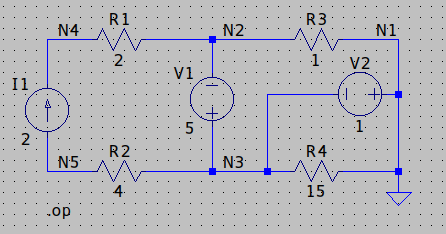
\includegraphics[width = 7cm]{example}
\caption{Odpowiadający schemat ideowy}
\end{figure}
\end{multicols}

\noindent Wynik działania programu:
\begin{lstlisting}
Potencjaly wezlowe:
        V(1) = 0 V
        V(2) = -6 V
        V(3) = -1 V
        V(4) = -2 V
        V(5) = -9 V
 
E1 - [3, 2]:
        V(E1) = -5 V
        I(E1) = 8 A
        P(E1) = -40 W
 
E2 - [3, 1]:
        V(E2) = 1 V
        I(E2) = -6.06667 A
        P(E2) = -6.06667 W
 
I1 - [5, 4]:
        V(I1) = 7 V
        I(I1) = -2 A
        P(I1) = -14 W
 
R1 - [4, 2]:
        V(R1) = -4 V
        I(R1) = -2 A
        P(R1) = 8 W
 
R2 - [5, 3]:
        V(R2) = 8 V
        I(R2) = 2 A
        P(R2) = 16 W
 
R3 - [1, 2]:
        V(R3) = -6 V
        I(R3) = -6 A
        P(R3) = 36 W
 
R4 - [3, 1]:
        V(R4) = 1 V
        I(R4) = 0.0666667 A
        P(R4) = 0.0666667 W
 
Moc calkowita: 60.0667 W.
\end{lstlisting}
\noindent Wynik działania programu LTSpice:
\begin{lstlisting}
       --- Operating Point ---
 
V(n2):   -6         voltage
V(n4):   -2         voltage
V(n3):   -1         voltage
V(n5):   -9         voltage
I(I1):   2          device_current
I(R4):   0.0666667  device_current
I(R3):   6          device_current
I(R2):   2          device_current
I(R1):   -2         device_current
I(V2):   -6.06667   device_current
I(V1):   -8         device_current
\end{lstlisting}

\noindent Jak można zauważyć, w obu przypadkach wyznaczone potencjały węzłowe i prądy płynące przez rezystory są takie same.

\newpage
\newgeometry{total={16cm, 25cm}} 
\subsection{Analiza AC --- filtr Sallen-Key}
Analiza AC filtru aktywnego II rzędu w topologii Salen-Key. Filtr został zaprojektowany\cite{okawa}, by częstotliwość odcięcia $f_c$ wynosiła w przybliżeniu 1kHz.

\begin{multicols}{2}
\begin{lstlisting}[caption=Netlista opisująca filtr]
Sallen-Key lowpass filter
 
OPA1 4 3 4
R1 1 2 16k
R2 2 3 16k
C1 2 4 0.01u
C2 3 0 0.01u
V1 1 0 0 ac 1
 
.ac dec 5 10 100k
.print ac V(4)
\end{lstlisting}

\columnbreak

\begin{figure}[H]
\centering
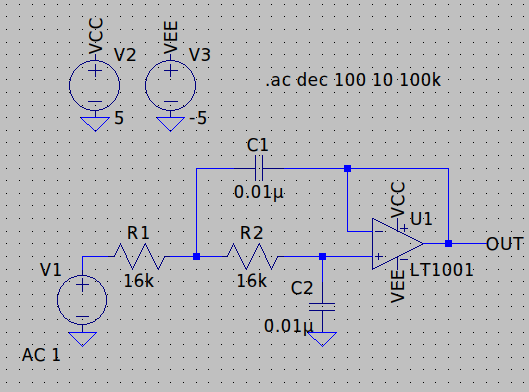
\includegraphics[height = 5cm]{sallen-ltspice-circ}
\caption{Schemat ideowy filtra}
\end{figure}
\end{multicols}


\begin{figure}[H]
\centering
\subfigure[Wynik symulacji w myspice]{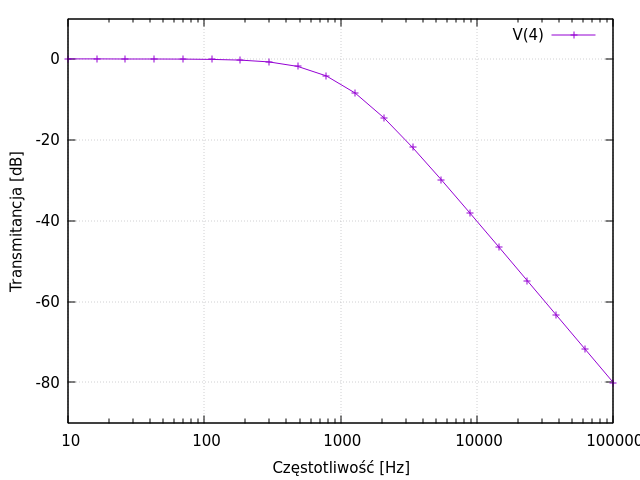
\includegraphics[height=6cm]{sallen}}
\hfill
\centering
\subfigure[Wynik symulacji w LTSpice]{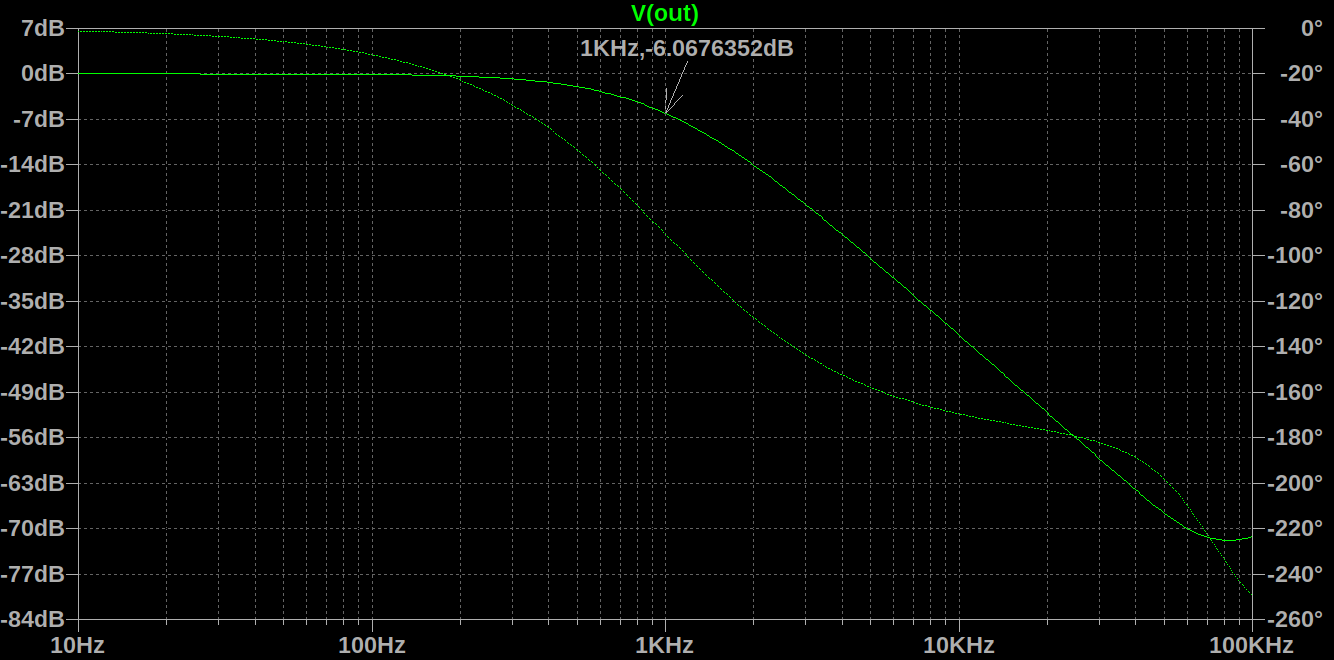
\includegraphics[height=6cm]{sallen-ltspice}}
\caption{Porównanie wyników symulacji z programem LTSpice}
\end{figure}

Porównując charakterystyki można zauważyć rozbieżność w wynikach jedynie dla wysokich częstotliwości ok. 100kHz. Jest to spowodowane
zastosowaniem nieidealnego wzmacniacza LT1001 w symulacji LTSpice.



\end{document}
